\begin{DoxyAuthor}{Author}
Craig Hesling (\href{mailto:craig@hesling.com}{\tt craig@hesling.\+com}) 
\end{DoxyAuthor}
\begin{DoxyDate}{Date}
Apr 6, 2014
\end{DoxyDate}
\hypertarget{index_intro_sec}{}\section{Introduction}\label{index_intro_sec}
T\+O\+D\+O\+: Stick introduction here... \hypertarget{index_expressions}{}\subsection{Expressions}\label{index_expressions}
Example\+: expression is $(1 + 2)$

\begin{center}

\begin{DoxyImageNoCaption}
  \mbox{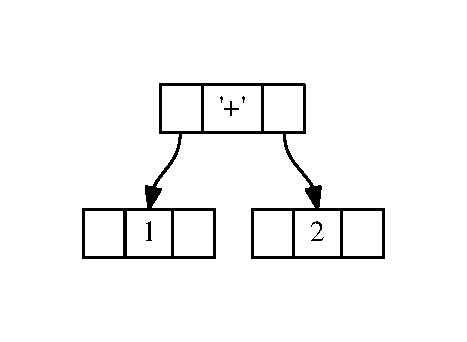
\includegraphics[width=\textwidth,height=\textheight/2,keepaspectratio=true]{dot_inline_dotgraph_2}}
\end{DoxyImageNoCaption}
\end{center}


Example\+: expression is $(1 + 2) + 3$

\begin{center}

\begin{DoxyImageNoCaption}
  \mbox{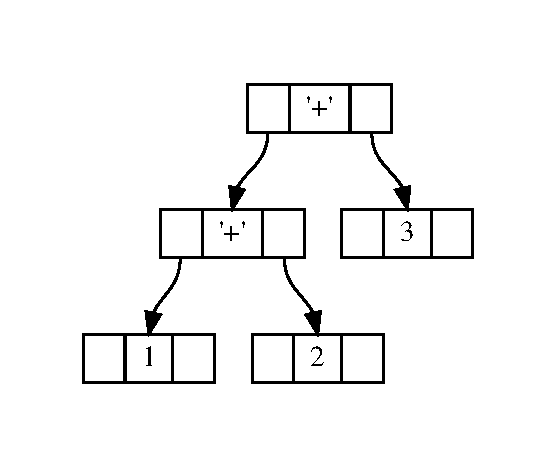
\includegraphics[width=\textwidth,height=\textheight/2,keepaspectratio=true]{dot_inline_dotgraph_3}}
\end{DoxyImageNoCaption}
\end{center}
\hypertarget{index_development}{}\section{Development}\label{index_development}
\hypertarget{index_quick_links}{}\subsection{Quick Links}\label{index_quick_links}

\begin{DoxyItemize}
\item Main library interface file for \hyperlink{expression_8h}{expression.\+h}
\item Main library implementation file for \hyperlink{expression_8c}{expression.\+c}
\end{DoxyItemize}\hypertarget{index_debug_info}{}\subsection{Helpful for Debugging}\label{index_debug_info}

\begin{DoxyItemize}
\item valgrind --tool=memcheck --track-\/origins=yes --undef-\/value-\/errors=yes --leak-\/check=full ./expr \char`\"{}1 + 2\char`\"{}
\item valgrind --tool=memcheck --track-\/origins=yes --undef-\/value-\/errors=yes --leak-\/check=full ./expr \char`\"{}1 + 2\char`\"{}
\item target remote $\vert$ /usr/lib/valgrind/../../bin/vgdb
\end{DoxyItemize}\hypertarget{index_future_changes}{}\subsection{Future Wish List}\label{index_future_changes}

\begin{DoxyItemize}
\item Make string\+\_\+to\+\_\+expression take a start index parameter. This would allow recursive calls to not need temporary string buffers and syntax errors to contain proper index numbers.
\item Handle floats and doubles
\item Handle builtin functions 
\end{DoxyItemize}